\begin{enumerate}[label=\thesection.\arabic*,ref=\thesection.\theenumi]
\numberwithin{equation}{enumi}
\numberwithin{figure}{enumi}
\numberwithin{table}{enumi}
\item
\label{12/12/3/1}
%\iffalse
\documentclass[journal,10pt,twocolumn]{article}
\usepackage{graphicx}
\usepackage[margin=0.5in]{geometry}
\usepackage{amsmath}
\usepackage{array}
\usepackage{booktabs}
\usepackage{listings}
\providecommand{\norm}[1]{\left\lVert#1\right\rVert}
\providecommand{\abs}[1]{\left\vert#1\right\vert}
\usepackage{enumerate}
\let\vec\mathbf
\newcommand{\myvec}[1]{\ensuremath{\myvec{#1}}}
\newcommand{\mydet}[1]{\ensuremath{\begin{vmatrix}#1\end{vmatrix}}}
\providecommand{\brak}[1]{\ensuremath{\left(#1\right)}}
\lstset{
frame=single,
breaklines=true,
columns=fullflexible
}
\title{\textbf{Matrix Assignment}}
\author{Mannava Venkatasai}
\date{September 2022}
\begin{document}
\maketitle
\raggedright \textbf{Problem Statement}: \vspace{3mm} \\
Two godowns A and B have grain capacity of 100 quintals and 50 quintals
respectively. They supply to 3 ration shops, D, E and F whose requirements are
60, 50 and 40 quintals respectively. The cost of transportation per quintal from
the godowns to the shops are given in the following table
\begin{table}[!ht]
	\centering
\begin{tabular}{|c|c|c|}
\hline
% \begin{tabularx}{\linewidth} {lX}
 From/to & A& B  \\ 
 \hline
 D & 6 & 4 \\  
 \hline
 E & 3  & 2 \\
 \hline
  F & 2.5 & 3 \\
 \hline
\end{tabular} 
\end{table} 
\vspace{5mm}
How should the supplies be transported in order that the transportation cost is minimum? What is the minimum cost?
\fi
%\\
%\solution
Let's assume that 
\begin{enumerate}
\item A supplies $x$ quintals grain to ration shop D.
\item A supplies $y$ quintals grain to ration shop E.
\item A will supply remaining grains 100-$x$-$y$ quintals to F.
\item B will supply 60-$x$ quintals grain to ration shop D. 
\item B will supply 50-$y$ quintals grain to ration shop E.
\item B will supply $x$+$y$-60 quintals grain to ration shop F.
\end{enumerate}
Total transportation cost is given by :
\begin{align}
P=2.5x+1.5y+410
\end{align}
Now, Since godown A can supply maximum 60 quintals to ration shop D and 50 quintals to ration shop E and have maximum 100 quintals capacity to supply.\vspace{2mm} \\ Also, if godown A supplies all 40 quintals to ration shop F, then remaining 60 quintals will be supplied to ration shop D and E and $x$ and $y$ is amount of grains. It can never be negative.  This leads to the following conditions
\begin{align}
x+y \le 100 \\
x \le 60 \\
y \le 50 \\
-x-y \le -60 \\
x \ge 0 \\
y \ge 0
\end{align}
\iffalse
The above equations in vector form is :
\begin{align}
\vec{A_1} = 
\myvec{
1 \\
1 \\
} \\
\vec{A_2} = 
\myvec{
1 \\
1 \\
} \\
\vec{A_3} = 
\myvec{
1 \\
0 \\
} \\
\vec{A_4} = 
\myvec{
0 \\
1 \\
} \\
\vec{x} = 
\myvec{
x \\
y \\
}
\end{align}
\begin{align}
\vec{A_1}\vec{x} \le 100
\end{align}
\begin{align}
\vec{A_2}\vec{x} \ge 60
\end{align}
\begin{align}
\vec{A_3}\vec{x} \le 60
\end{align}
\begin{align}
\vec{A_4}\vec{x} \le 50
\end{align}
which can be expressed in vector form as
\fi
The optimization problem can then be expressed as
\begin{align}
	P=\max_{\vec{x}}\myvec{2.5 & 1.5}\vec{x}+410
	\\
	s.t. \quad
 \myvec{1 &1 \\ -1 & -1 \\ -1 & 0 \\ 0 & -1 \\} \vec{x}\preceq \myvec{100 \\ -60 \\ -60 \\ -50}
\end{align}
yielding
\begin{align}
	P = 510, 
\vec{x} = 
\myvec{
10 \\
50 \\
}
\end{align}
Hence,
\begin{enumerate}
\item The minimum transportation cost is : 510 /-
\item A supplies 10 quintals grain to ration shop D.
\item A supplies 50 quintals grain to ration shop E.
\item A supplies 40 quintals grain to ration shop F.
\item A supplies 50 quintals grain to ration shop D.
\item A supplies 0 quintals grain to ration shop E.
\item A supplies 0 quintals grain to ration shop F.
\end{enumerate}

\item
\label{12/12/3/2}
%\iffalse
\documentclass[journal,10pt,twocolumn]{article}
\usepackage{graphicx}
\usepackage[margin=0.5in]{geometry}
\usepackage{amsmath}
\usepackage{array}
\usepackage{booktabs}
\usepackage{listings}
\providecommand{\norm}[1]{\left\lVert#1\right\rVert}
\providecommand{\abs}[1]{\left\vert#1\right\vert}
\usepackage{enumerate}
\let\vec\mathbf
\newcommand{\myvec}[1]{\ensuremath{\myvec{#1}}}
\newcommand{\mydet}[1]{\ensuremath{\begin{vmatrix}#1\end{vmatrix}}}
\providecommand{\brak}[1]{\ensuremath{\left(#1\right)}}
\lstset{
frame=single,
breaklines=true,
columns=fullflexible
}
\title{\textbf{Matrix Assignment}}
\author{Mannava Venkatasai}
\date{September 2022}
\begin{document}
\maketitle
\raggedright \textbf{Problem Statement}: \vspace{3mm} \\
Two godowns A and B have grain capacity of 100 quintals and 50 quintals
respectively. They supply to 3 ration shops, D, E and F whose requirements are
60, 50 and 40 quintals respectively. The cost of transportation per quintal from
the godowns to the shops are given in the following table
\begin{table}[!ht]
	\centering
\begin{tabular}{|c|c|c|}
\hline
% \begin{tabularx}{\linewidth} {lX}
 From/to & A& B  \\ 
 \hline
 D & 6 & 4 \\  
 \hline
 E & 3  & 2 \\
 \hline
  F & 2.5 & 3 \\
 \hline
\end{tabular} 
\end{table} 
\vspace{5mm}
How should the supplies be transported in order that the transportation cost is minimum? What is the minimum cost?
\fi
%\\
%\solution
Let's assume that 
\begin{enumerate}
\item A supplies $x$ quintals grain to ration shop D.
\item A supplies $y$ quintals grain to ration shop E.
\item A will supply remaining grains 100-$x$-$y$ quintals to F.
\item B will supply 60-$x$ quintals grain to ration shop D. 
\item B will supply 50-$y$ quintals grain to ration shop E.
\item B will supply $x$+$y$-60 quintals grain to ration shop F.
\end{enumerate}
Total transportation cost is given by :
\begin{align}
P=2.5x+1.5y+410
\end{align}
Now, Since godown A can supply maximum 60 quintals to ration shop D and 50 quintals to ration shop E and have maximum 100 quintals capacity to supply.\vspace{2mm} \\ Also, if godown A supplies all 40 quintals to ration shop F, then remaining 60 quintals will be supplied to ration shop D and E and $x$ and $y$ is amount of grains. It can never be negative.  This leads to the following conditions
\begin{align}
x+y \le 100 \\
x \le 60 \\
y \le 50 \\
-x-y \le -60 \\
x \ge 0 \\
y \ge 0
\end{align}
\iffalse
The above equations in vector form is :
\begin{align}
\vec{A_1} = 
\myvec{
1 \\
1 \\
} \\
\vec{A_2} = 
\myvec{
1 \\
1 \\
} \\
\vec{A_3} = 
\myvec{
1 \\
0 \\
} \\
\vec{A_4} = 
\myvec{
0 \\
1 \\
} \\
\vec{x} = 
\myvec{
x \\
y \\
}
\end{align}
\begin{align}
\vec{A_1}\vec{x} \le 100
\end{align}
\begin{align}
\vec{A_2}\vec{x} \ge 60
\end{align}
\begin{align}
\vec{A_3}\vec{x} \le 60
\end{align}
\begin{align}
\vec{A_4}\vec{x} \le 50
\end{align}
which can be expressed in vector form as
\fi
The optimization problem can then be expressed as
\begin{align}
	P=\max_{\vec{x}}\myvec{2.5 & 1.5}\vec{x}+410
	\\
	s.t. \quad
 \myvec{1 &1 \\ -1 & -1 \\ -1 & 0 \\ 0 & -1 \\} \vec{x}\preceq \myvec{100 \\ -60 \\ -60 \\ -50}
\end{align}
yielding
\begin{align}
	P = 510, 
\vec{x} = 
\myvec{
10 \\
50 \\
}
\end{align}
Hence,
\begin{enumerate}
\item The minimum transportation cost is : 510 /-
\item A supplies 10 quintals grain to ration shop D.
\item A supplies 50 quintals grain to ration shop E.
\item A supplies 40 quintals grain to ration shop F.
\item A supplies 50 quintals grain to ration shop D.
\item A supplies 0 quintals grain to ration shop E.
\item A supplies 0 quintals grain to ration shop F.
\end{enumerate}

\item
\label{12/12/3/3}
\iffalse
\documentclass{article}
% Language setting
% Replace `english' with e.g. `spanish' to change the document language
\usepackage[english]{babel}
% Set page size and margins
% Replace `letterpaper' with `a4paper' for UK/EU standard size
\usepackage[letterpaper,top=2cm,bottom=2cm,left=3cm,right=3cm,marginparwidth=1.75cm]{geometry}
% Useful packages
\usepackage{multicol}
\usepackage{amsmath}
\usepackage{amssymb}
\usepackage{graphicx}
\usepackage[framemethod=tikz]{mdframed}
\usepackage{array}
\usepackage{blindtext}
%\usepackage[paperwidth=10cm]{geometry}
\usepackage{tkz-euclide}
%\usepackage{tikz}
\usetikzlibrary{
  circuits.logic,
  circuits.logic.US,
  positioning
}

\usepackage[colorlinks=true, allcolors=blue]{hyperref}
\newcommand{\myvec}[1]{\ensuremath{\begin{pmatrix}#1\end{pmatrix}}}
\providecommand{\norm}[1]{\left\lVert#1\right\rVert}
\let\vec\mathbf
\title{Optimization Assignment-1}
\author{Anusha Jella}
\begin{document}
\maketitle
\newtheorem{theorem}{Theorem}[section]
\begin{multicols}{2}

\paragraph{\begin{flushleft}\textbf{Problem: }
	\fi
A dietician wishes to mix together two kinds of food X and Y in such away that the mixture contains atleast 10 units of vitamin A ,12 units of vitamin B and 8 units of vitamin C .The vitamin contents of one kg food is given below
\iffalse
\end{flushleft}}
\resizebox{6.5cm}{!}
{
	\fi
	\begin{table}[!ht]
		\centering
\begin{tabular}{|c|c|c|c|}
	\hline
	\textbf{Food}&\textbf{Vitamin A}&\textbf{Vitamin B}&\textbf{Vitamin C}\\
	\hline
	\textbf{X}&1&2&3\\
	\hline
	\textbf{Y}&2&2&1\\
	\hline
\end{tabular}
		\caption{}
		\label{fig:12/12/3/3}
\end{table}
One kg of food X costs Rs 16 and one kg of food Y costs Rs 20. Find the least
cost of the mixture which will produce the required diet.
\\
\solution
	\iffalse
	\begin{figure}[!ht]
		\centering
		\includegraphics[width=\columnwidth]{12/12/3/3/figs/opt_fig1.pdf}
		\caption{}
		\label{fig:12/12/3/3}
  	\end{figure}
\end{flushleft}
\includegraphics[scale=0.5]{opt_fig1.pdf} 
\section*{Solution}
\begin{flushleft}
Let mixture contains x units of food X,y units of food Y.\\
According to given problem, problem can be formulated as,\\
\end{flushleft}
\begin{align}
P=min(16x+20y)
\end{align}
where P is minimum cost of mixture.\\
for Vitamin A
\begin{align}
x+2y \geq10
\end{align}
for Vitamin B
\begin{align}
2x+2y \geq 12
\end{align}
for Vitamin C
\begin{align}
3x+y \geq 8
\end{align}
mixture contains both X,Y so,
\begin{align}
x\geq0,y\geq0
\end{align}
eq 1 and 2 to 5 can be expressed in vector form as
\begin{align*}
\vec{P}=min\myvec{16 \hspace{0.2cm}20}\vec{x}\\
\myvec{1 \hspace{0.2cm} 2\\
       2 \hspace{0.2cm} 2\\
       3 \hspace{0.2cm} 1\\
       1 \hspace{0.2cm}0\\
       0 \hspace{0.2cm} 1}\vec{x}\geq \myvec{10 \\12\\8\\0\\0}
\end{align*}
Solving above equations using cvxpy, we get\\
\vspace{0.1cm}\\
$P_{min}$=120\\
$\vec{x}$=$\myvec{2\\4}$
\end{multicols}{2}
\end{document}
\fi

\item
\label{12/12/3/4}
\iffalse
\documentclass[journal,12pt,twocolumn]{IEEEtran}

\usepackage[utf8]{inputenc}
\usepackage{kvmap}
\usepackage{graphics} 

\usepackage{setspace}
\usepackage{gensymb}

\singlespacing


\usepackage{amsthm}

\usepackage{mathrsfs}
\usepackage{txfonts}
\usepackage{stfloats}
\usepackage{bm}
\usepackage{cite}
\usepackage{cases}
\usepackage{subfig}

\usepackage{longtable}
\usepackage{multirow}

\usepackage{enumitem}
\usepackage{mathtools}
\usepackage{steinmetz}
\usepackage{tikz}
\usepackage{circuitikz}
\usepackage{verbatim}
\usepackage{tfrupee}
\usepackage[breaklinks=true]{hyperref}
\usepackage{graphicx}
\usepackage{tkz-euclide}
\usepackage{float}

\usetikzlibrary{calc,math}
\usepackage{listings}
    \usepackage{color}                                            %%
    \usepackage{array}                                            %%
    \usepackage{longtable}                                        %%
    \usepackage{calc}                                             %%
    \usepackage{multirow}                                         %%
    \usepackage{hhline}                                           %%
    \usepackage{ifthen}                                           %%
    \usepackage{lscape}     
\usepackage{multicol}
\usepackage{chngcntr}

\DeclareMathOperator*{\Res}{Res}

\renewcommand\thesection{\arabic{section}}
\renewcommand\thesubsection{\thesection.\arabic{subsection}}
\renewcommand\thesubsubsection{\thesubsection.\arabic{subsubsection}}

\renewcommand\thesectiondis{\arabic{section}}
\renewcommand\thesubsectiondis{\thesectiondis.\arabic{subsection}}
\renewcommand\thesubsubsectiondis{\thesubsectiondis.\arabic{subsubsection}}


\hyphenation{op-tical net-works semi-conduc-tor}
\def\inputGnumericTable{}                                 %%

\lstset{
%language=C,
frame=single, 
breaklines=true,
columns=fullflexible
}
\begin{document}


\newtheorem{theorem}{Theorem}[section]
\newtheorem{problem}{Problem}
\newtheorem{proposition}{Proposition}[section]
\newtheorem{lemma}{Lemma}[section]
\newtheorem{corollary}[theorem]{Corollary}
\newtheorem{example}{Example}[section]
\newtheorem{definition}[problem]{Definition}

\newcommand{\BEQA}{\begin{eqnarray}}
\newcommand{\EEQA}{\end{eqnarray}}
\newcommand{\define}{\stackrel{\triangle}{=}}
\newcommand\hlight[1]{\tikz[overlay, remember picture,baseline=-\the\dimexpr\fontdimen22\textfont2\relax]\node[rectangle,fill=blue!50,rounded corners,fill opacity = 0.2,draw,thick,text opacity =1] {$#1$};}
\bibliographystyle{IEEEtran}
\providecommand{\mbf}{\mathbf}
\providecommand{\pr}[1]{\ensuremath{\Pr\left(#1\right)}}
\providecommand{\qfunc}[1]{\ensuremath{Q\left(#1\right)}}
\providecommand{\sbrak}[1]{\ensuremath{{}\left[#1\right]}}
\providecommand{\lsbrak}[1]{\ensuremath{{}\left[#1\right.}}
\providecommand{\rsbrak}[1]{\ensuremath{{}\left.#1\right]}}
\providecommand{\brak}[1]{\ensuremath{\left(#1\right)}}
\providecommand{\lbrak}[1]{\ensuremath{\left(#1\right.}}
\providecommand{\rbrak}[1]{\ensuremath{\left.#1\right)}}
\providecommand{\cbrak}[1]{\ensuremath{\left\{#1\right\}}}
\providecommand{\lcbrak}[1]{\ensuremath{\left\{#1\right.}}
\providecommand{\rcbrak}[1]{\ensuremath{\left.#1\right\}}}
\theoremstyle{remark}
\newtheorem{rem}{Remark}
\newcommand{\sgn}{\mathop{\mathrm{sgn}}}
\providecommand{\abs}[1]{\left\vert#1\right\vert}
\providecommand{\res}[1]{\Res\displaylimits_{#1}} 
\providecommand{\norm}[1]{$\left\lVert#1\right\rVert$}
%\providecommand{\norm}[1]{\lVert#1\rVert}
\providecommand{\mtx}[1]{\mathbf{#1}}
\providecommand{\mean}[1]{E\left[ #1 \right]}
\providecommand{\fourier}{\overset{\mathcal{F}}{ \rightleftharpoons}}
%\providecommand{\hilbert}{\overset{\mathcal{H}}{ \rightleftharpoons}}
\providecommand{\system}{\overset{\mathcal{H}}{ \longleftrightarrow}}
	%\newcommand{\solution}[2]{\textbf{Solution:}{#1}}
\newcommand{\solution}{\noindent \textbf{Solution: }}
\newcommand{\cosec}{\,\text{cosec}\,}
\providecommand{\dec}[2]{\ensuremath{\overset{#1}{\underset{#2}{\gtrless}}}}
\newcommand{\myvec}[1]{\ensuremath{\begin{pmatrix}#1\end{pmatrix}}}
\newcommand{\mydet}[1]{\ensuremath{\begin{vmatrix}#1\end{vmatrix}}}
\numberwithin{equation}{subsection}
\makeatletter
\@addtoreset{figure}{problem}
\makeatother
\let\StandardTheFigure\thefigure
\let\vec\mathbf
\renewcommand{\thefigure}{\theproblem}
\def\putbox#1#2#3{\makebox[0in][l]{\makebox[#1][l]{}\raisebox{\baselineskip}[0in][0in]{\raisebox{#2}[0in][0in]{#3}}}}
     \def\rightbox#1{\makebox[0in][r]{#1}}
     \def\centbox#1{\makebox[0in]{#1}}
     \def\topbox#1{\raisebox{-\baselineskip}[0in][0in]{#1}}
     \def\midbox#1{\raisebox{-0.5\baselineskip}[0in][0in]{#1}}
\vspace{3cm}
\title{\textbf{Optimization-Linear} }
\author{Surabhi Seetha}
\maketitle
\newpage
\bigskip
\renewcommand{\thefigure}{\theenumi}
\renewcommand{\thetable}{\theenumi}
Get Python code for the figure from 
\begin{lstlisting}
https://github.com/SurabhiSeetha/Fwciith2022/tree/main/Assignment%201/codes/src
\end{lstlisting}
Get LaTex code from
\begin{lstlisting}
https://github.com/SurabhiSeetha/Fwciith2022/tree/main/avr%20gcc
\end{lstlisting}
%
\section{Question-Class 12, Miscellaneous, Q(4)}
\fi
A manufacturer makes two types of toys A and B.Three machines are needed for this purpose and the time(in minutes)required for each toy on the machines is given below
\begin{table}[!ht]
	\centering
\begin{tabular}{|c|c|c|c|}
\hline
\textbf{Types of Toys} & \textbf{I} & \textbf{II} & \textbf{III}\\
\hline
A & 12 & 18 & 6\\
\hline
B & 6 & 0 & 9\\
\hline
\end{tabular}
\end{table}
\vspace{0.4cm}\\
\raggedright
Each machine is available for a maximum 6 hours per day. If the profit on each toy of type A is Rs.7.50 and that on each toy of type B is Rs.5, show that 15 toys of type A and 30 type B should be manufactured in a day to get maximum profit.
\\
\solution
	\begin{figure}[!ht]
		\centering
		\includegraphics[width=\columnwidth]{12/12/3/4/figs/optlinear1.png}
		\caption{}
		\label{fig:12/12/3/4}
  	\end{figure}
	\iffalse
\section{Solution}
\includegraphics[width=0.5\textwidth]{optlinear1.png}\\
From the figure we get, four points A(0,40), B(15,30),C(20,20),D(20,0)\\
We get these four points through the equations derived and by converting the minutes time into hours from the table above as,\\
\vspace{0.25cm}
\centering
$12x+6y\leq{360}$\\
$18x\leq{360}$\\
$6x+9y\leq{360}$\\
\raggedright
simplified as,\\
\centering
$2x+y\leq1$\\
$3x\leq{1}$\\
$2x+3y\leq{2}$\\
\raggedright
x and y are the profits of A and B\\
\raggedright
{Now,}\\
\centering
\vspace{0.25cm}
$Z_{max}=7.50x+5y$\\
\raggedright
\fi
The given information can be framed as the optimization problem 
\begin{align}
 Z = \max_{\vec{x}} \myvec{7.50&5} \vec{x}\\
\myvec{2&1\\3&0\\2&3}\vec{x} \preceq \myvec{1\\1\\2}\\
 \vec{x} \succeq  \vec{0}
\end{align}
Solving the above equations using cvxpy, we obtain 
\begin{align}
Z_{max} = Rs. 262.50,
\vec{x} = \myvec{15\\30} 
\end{align}


\item
\label{12/12/3/5}
\iffalse
\documentclass[10pt,twocolumn]{article}
\usepackage{graphicx}
\usepackage[margin=0.5in]{geometry}
\usepackage[cmex10]{amsmath}
\usepackage{array}
\usepackage{booktabs}
\usepackage{mathtools}
\title{\textbf{Optimization Assignment - 1}}
\author{A L U R U A J A Y}
\date{September 2022}


\providecommand{\norm}[1]{\left\lVert#1\right\rVert}
\providecommand{\abs}[1]{\left\vert#1\right\vert}
\let\vec\mathbf
\newcommand{\myvec}[1]{\ensuremath{\begin{pmatrix}#1\end{pmatrix}}}
\newcommand{\mydet}[1]{\ensuremath{\begin{vmatrix}#1\end{vmatrix}}}
\providecommand{\brak}[1]{\ensuremath{\left(#1\right)}}
\providecommand{\lbrak}[1]{\ensuremath{\left(#1\right.}}
\providecommand{\rbrak}[1]{\ensuremath{\left.#1\right)}}
\providecommand{\sbrak}[1]{\ensuremath{{}\left[#1\right]}}

\begin{document}

\maketitle
\paragraph{\textit{Problem Statement} -
An aeroplane can carry a maximum of 200 passengers.A profit of Rs.1000 is made on each executive class ticket and a profit of Rs.600 is made on each economy class ticket. The airline reserves at least 20 seats for executive class. However, at least 4 times as many passengers prefer to travel by economy class than by the executive class. Determine how many tickets of each type must be sold in order to maximise the profit for the airline. What is the maximum profit? 
\fi
%\\
%\solution
\iffalse
\section{Solution}
Let Number of Executive class ticket sold be x
\vspace{0.3cm}\\
Let Number of Economy class ticket sold be y
\vspace{0.3cm}\\
According to Question
\vspace{0.3cm}\\
Aeroplane can carry maximum 200 passengers
\begin{align}
    x+y \leq 200
    \vspace{0.3cm}\\
    \myvec{1\\1}\vec{x}\leq 200
\end{align}
Since, atleast 20 tickets is reserves for executive class
\begin{align}
  x \ge 20  
  \vspace{0.3cm}\\
\myvec{1\\0}\vec{x}\ge 20
\end{align}
Since the number of tickets for economy class should be at least 4 times the executive class
\begin{align}
    y - 4x \ge 0
    \vspace{0.3cm}\\
     \myvec{-4\\1}\vec{x}\ge 0
\end{align}
Also, the number of tickets can't be negative,so
\begin{align}
    x \ge 0 \And y\ge 0
    \vspace{0.3cm}\\
    \myvec{1 \\ 0} \vec{x} \ge 0
      \vspace{0.4cm}\\
    \myvec{0 \\ 1} \vec{y} \ge 0
\end{align}
\begin{flushleft}
The above equations in vector form is :
\begin{align}
\vec{A_1} = 
\begin{pmatrix}
1 \\
1 \\
\end{pmatrix} \\
\vec{A_2} = 
\begin{pmatrix}
1 \\
0 \\
\end{pmatrix} \\
\vec{A_3} = 
\begin{pmatrix}
-4 \\
1 \\
\end{pmatrix} \\
\vec{A_4} = 
\begin{pmatrix}
1 \\
0 \\
\end{pmatrix} \\
\vec{A_5} = 
\begin{pmatrix}
0 \\
1 \\
\end{pmatrix} \\
\end{align}
\begin{flushleft}
which can be expressed in vector form as
\end{flushleft}
\begin{align}
 \myvec{-1 &-1 \\ 1 & 0 \\ -4 & 1 \\} \vec{x}\ge \myvec{200 \\ 20 \\ 0}
\end{align}
\fi
Let $P$ be the maximum number of tickets of each type must be sold in order to maximise the profit for the airline . The problem can be formulated as
\begin{align}
	P = \max_{\vec{x}}\myvec{1 & 1}\vec{x}
	\\
	s.t. \quad
 \myvec{-1 &-1 \\ 1 & 0 \\ -4 & 1 \\} \vec{x}\succeq \myvec{200 \\ 20 \\ 0}
\end{align}
yielding
\begin{align}
	P_{max} = 136000, 
	\vec{x} = \myvec{40 \\ 160}
\end{align}
	\begin{figure}[!ht]
		\centering
		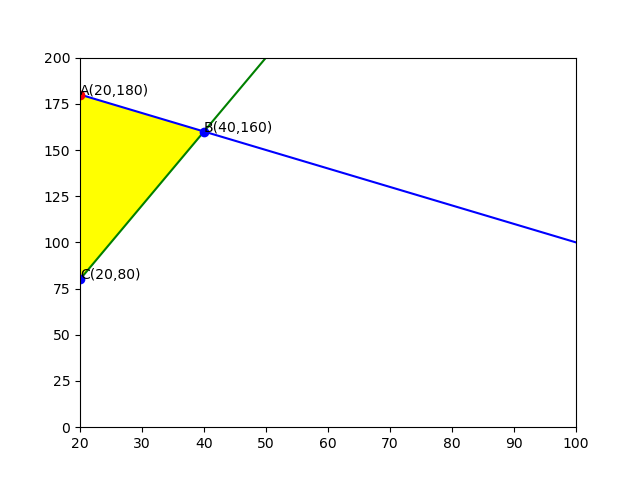
\includegraphics[width=\columnwidth]{12/12/3/5/figs/opt.png}
		\caption{}
		\label{fig:12/12/3/5}
  	\end{figure}
\iffalse
\begin{figure}[h]
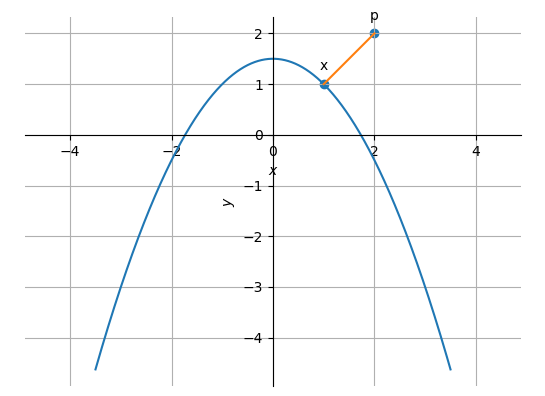
\includegraphics[scale=0.3]{opt.png}
\caption{Graph}
\label{fig:Graph}
\end{figure}

\end{document}
\fi







\item
\label{12/12/3/6}
\iffalse
\documentclass[journal,10pt,twocolumn]{article}
\usepackage{graphicx}
\usepackage[margin=0.5in]{geometry}
\usepackage{amsmath}
\usepackage{array}
\usepackage{booktabs}
\usepackage{listings}
\providecommand{\norm}[1]{\left\lVert#1\right\rVert}
\providecommand{\abs}[1]{\left\vert#1\right\vert}
\usepackage{enumerate}
\let\vec\mathbf
\newcommand{\myvec}[1]{\ensuremath{\myvec{#1}}}
\newcommand{\mydet}[1]{\ensuremath{\begin{vmatrix}#1\end{vmatrix}}}
\providecommand{\brak}[1]{\ensuremath{\left(#1\right)}}
\lstset{
frame=single,
breaklines=true,
columns=fullflexible
}
\title{\textbf{Matrix Assignment}}
\author{Mannava Venkatasai}
\date{September 2022}
\begin{document}
\maketitle
\raggedright \textbf{Problem Statement}: \vspace{3mm} \\
Two godowns A and B have grain capacity of 100 quintals and 50 quintals
respectively. They supply to 3 ration shops, D, E and F whose requirements are
60, 50 and 40 quintals respectively. The cost of transportation per quintal from
the godowns to the shops are given in the following table
\begin{table}[!ht]
	\centering
\begin{tabular}{|c|c|c|}
\hline
% \begin{tabularx}{\linewidth} {lX}
 From/to & A& B  \\ 
 \hline
 D & 6 & 4 \\  
 \hline
 E & 3  & 2 \\
 \hline
  F & 2.5 & 3 \\
 \hline
\end{tabular} 
\end{table} 
\vspace{5mm}
How should the supplies be transported in order that the transportation cost is minimum? What is the minimum cost?
\fi
%\\
%\solution
Let's assume that 
\begin{enumerate}
\item A supplies $x$ quintals grain to ration shop D.
\item A supplies $y$ quintals grain to ration shop E.
\item A will supply remaining grains 100-$x$-$y$ quintals to F.
\item B will supply 60-$x$ quintals grain to ration shop D. 
\item B will supply 50-$y$ quintals grain to ration shop E.
\item B will supply $x$+$y$-60 quintals grain to ration shop F.
\end{enumerate}
Total transportation cost is given by :
\begin{align}
P=2.5x+1.5y+410
\end{align}
Now, Since godown A can supply maximum 60 quintals to ration shop D and 50 quintals to ration shop E and have maximum 100 quintals capacity to supply.\vspace{2mm} \\ Also, if godown A supplies all 40 quintals to ration shop F, then remaining 60 quintals will be supplied to ration shop D and E and $x$ and $y$ is amount of grains. It can never be negative.  This leads to the following conditions
\begin{align}
x+y \le 100 \\
x \le 60 \\
y \le 50 \\
-x-y \le -60 \\
x \ge 0 \\
y \ge 0
\end{align}
\iffalse
The above equations in vector form is :
\begin{align}
\vec{A_1} = 
\myvec{
1 \\
1 \\
} \\
\vec{A_2} = 
\myvec{
1 \\
1 \\
} \\
\vec{A_3} = 
\myvec{
1 \\
0 \\
} \\
\vec{A_4} = 
\myvec{
0 \\
1 \\
} \\
\vec{x} = 
\myvec{
x \\
y \\
}
\end{align}
\begin{align}
\vec{A_1}\vec{x} \le 100
\end{align}
\begin{align}
\vec{A_2}\vec{x} \ge 60
\end{align}
\begin{align}
\vec{A_3}\vec{x} \le 60
\end{align}
\begin{align}
\vec{A_4}\vec{x} \le 50
\end{align}
which can be expressed in vector form as
\fi
The optimization problem can then be expressed as
\begin{align}
	P=\max_{\vec{x}}\myvec{2.5 & 1.5}\vec{x}+410
	\\
	s.t. \quad
 \myvec{1 &1 \\ -1 & -1 \\ -1 & 0 \\ 0 & -1 \\} \vec{x}\preceq \myvec{100 \\ -60 \\ -60 \\ -50}
\end{align}
yielding
\begin{align}
	P = 510, 
\vec{x} = 
\myvec{
10 \\
50 \\
}
\end{align}
Hence,
\begin{enumerate}
\item The minimum transportation cost is : 510 /-
\item A supplies 10 quintals grain to ration shop D.
\item A supplies 50 quintals grain to ration shop E.
\item A supplies 40 quintals grain to ration shop F.
\item A supplies 50 quintals grain to ration shop D.
\item A supplies 0 quintals grain to ration shop E.
\item A supplies 0 quintals grain to ration shop F.
\end{enumerate}

\item
\label{12/12/3/7}
%\iffalse
\documentclass[journal,10pt,twocolumn]{article}
\usepackage{graphicx}
\usepackage[margin=0.5in]{geometry}
\usepackage{amsmath}
\usepackage{array}
\usepackage{booktabs}
\usepackage{listings}
\providecommand{\norm}[1]{\left\lVert#1\right\rVert}
\providecommand{\abs}[1]{\left\vert#1\right\vert}
\usepackage{enumerate}
\let\vec\mathbf
\newcommand{\myvec}[1]{\ensuremath{\myvec{#1}}}
\newcommand{\mydet}[1]{\ensuremath{\begin{vmatrix}#1\end{vmatrix}}}
\providecommand{\brak}[1]{\ensuremath{\left(#1\right)}}
\lstset{
frame=single,
breaklines=true,
columns=fullflexible
}
\title{\textbf{Matrix Assignment}}
\author{Mannava Venkatasai}
\date{September 2022}
\begin{document}
\maketitle
\raggedright \textbf{Problem Statement}: \vspace{3mm} \\
Two godowns A and B have grain capacity of 100 quintals and 50 quintals
respectively. They supply to 3 ration shops, D, E and F whose requirements are
60, 50 and 40 quintals respectively. The cost of transportation per quintal from
the godowns to the shops are given in the following table
\begin{table}[!ht]
	\centering
\begin{tabular}{|c|c|c|}
\hline
% \begin{tabularx}{\linewidth} {lX}
 From/to & A& B  \\ 
 \hline
 D & 6 & 4 \\  
 \hline
 E & 3  & 2 \\
 \hline
  F & 2.5 & 3 \\
 \hline
\end{tabular} 
\end{table} 
\vspace{5mm}
How should the supplies be transported in order that the transportation cost is minimum? What is the minimum cost?
\fi
%\\
%\solution
Let's assume that 
\begin{enumerate}
\item A supplies $x$ quintals grain to ration shop D.
\item A supplies $y$ quintals grain to ration shop E.
\item A will supply remaining grains 100-$x$-$y$ quintals to F.
\item B will supply 60-$x$ quintals grain to ration shop D. 
\item B will supply 50-$y$ quintals grain to ration shop E.
\item B will supply $x$+$y$-60 quintals grain to ration shop F.
\end{enumerate}
Total transportation cost is given by :
\begin{align}
P=2.5x+1.5y+410
\end{align}
Now, Since godown A can supply maximum 60 quintals to ration shop D and 50 quintals to ration shop E and have maximum 100 quintals capacity to supply.\vspace{2mm} \\ Also, if godown A supplies all 40 quintals to ration shop F, then remaining 60 quintals will be supplied to ration shop D and E and $x$ and $y$ is amount of grains. It can never be negative.  This leads to the following conditions
\begin{align}
x+y \le 100 \\
x \le 60 \\
y \le 50 \\
-x-y \le -60 \\
x \ge 0 \\
y \ge 0
\end{align}
\iffalse
The above equations in vector form is :
\begin{align}
\vec{A_1} = 
\myvec{
1 \\
1 \\
} \\
\vec{A_2} = 
\myvec{
1 \\
1 \\
} \\
\vec{A_3} = 
\myvec{
1 \\
0 \\
} \\
\vec{A_4} = 
\myvec{
0 \\
1 \\
} \\
\vec{x} = 
\myvec{
x \\
y \\
}
\end{align}
\begin{align}
\vec{A_1}\vec{x} \le 100
\end{align}
\begin{align}
\vec{A_2}\vec{x} \ge 60
\end{align}
\begin{align}
\vec{A_3}\vec{x} \le 60
\end{align}
\begin{align}
\vec{A_4}\vec{x} \le 50
\end{align}
which can be expressed in vector form as
\fi
The optimization problem can then be expressed as
\begin{align}
	P=\max_{\vec{x}}\myvec{2.5 & 1.5}\vec{x}+410
	\\
	s.t. \quad
 \myvec{1 &1 \\ -1 & -1 \\ -1 & 0 \\ 0 & -1 \\} \vec{x}\preceq \myvec{100 \\ -60 \\ -60 \\ -50}
\end{align}
yielding
\begin{align}
	P = 510, 
\vec{x} = 
\myvec{
10 \\
50 \\
}
\end{align}
Hence,
\begin{enumerate}
\item The minimum transportation cost is : 510 /-
\item A supplies 10 quintals grain to ration shop D.
\item A supplies 50 quintals grain to ration shop E.
\item A supplies 40 quintals grain to ration shop F.
\item A supplies 50 quintals grain to ration shop D.
\item A supplies 0 quintals grain to ration shop E.
\item A supplies 0 quintals grain to ration shop F.
\end{enumerate}

\item
\label{12/12/3/8}
\iffalse
\documentclass[journal,10pt,twocolumn]{article}
\usepackage{graphicx}
\usepackage[margin=0.5in]{geometry}
\usepackage[cmex10]{amsmath}
\usepackage{array}
\usepackage{booktabs}
\usepackage{mathtools}
\title{\textbf{Optimization Assignment - 1}}
\author{Akana Sai Kumar}
\date{Oct 2022}


\providecommand{\norm}[1]{\left\lVert#1\right\rVert}
\providecommand{\abs}[1]{\left\vert#1\right\vert}
\let\vec\mathbf
\newcommand{\myvec}[1]{\ensuremath{\begin{pmatrix}#1\end{pmatrix}}}
\newcommand{\mydet}[1]{\ensuremath{\begin{vmatrix}#1\end{vmatrix}}}
\providecommand{\brak}[1]{\ensuremath{\left(#1\right)}}
\providecommand{\lbrak}[1]{\ensuremath{\left(#1\right.}}
\providecommand{\rbrak}[1]{\ensuremath{\left.#1\right)}}
\providecommand{\sbrak}[1]{\ensuremath{{}\left[#1\right]}}

\begin{document}

\maketitle
\paragraph{\textit{Problem Statement} -
\fi
A fruit grower can use two types of fertilizer in his garden, brand P and brand Q.The amounts (in kg) of nitrogen, phosphoric acid, potash, and chlorine in a bag of each brand are given in the table. Tests indicate that the garden needs at least 240 kg of phosphoric acid, at least 270 kg of potash and at most 310 kg of chlorine.
If the grower wants to minimise the amount of nitrogen added to the garden, how many bags of each brand should be used? What is the minimum amount of nitrogen added in the garden? 
\\
\solution
The given information is summarized in Table
		\ref{table:12/12/3/8}.
\begin{table}[!ht]
	\centering
\begin{tabular}{|c|c|c|}
\hline
 Kg per bag & Brand P& Brand Q  \\ 
 \hline
 Nitrogen & 3 & 3.5 \\  
 \hline
 Phosphoric acid & 1  & 2 \\
 \hline
  Potash & 3 & 1.5 \\
 \hline
 Chlorine & 1.5 & 2\\
 \hline
\end{tabular} 
	\caption{}
		\label{table:12/12/3/8}
\end{table} 

	\begin{figure}[!ht]
		\centering
		\includegraphics[width=\columnwidth]{12/12/3/8/figs/op.pdf}
		\caption{}
		\label{fig:12/12/3/8}
  	\end{figure}
\iffalse
\section*{\large Solution}
Let x be the bags of Brand P, y be  the bags of Brand Q. The problem can be formulated as
\begin{align}
	P = \min_{x,y} \vec{x}\\
	2x + y \geq 180\\
	x + 2y \geq 240\\
	1.5x + 2y \leq 310\\
	x \geq 0\\
	y \geq 0
\end{align}
which can be expressed in vector form as
\fi
The given problem can be expressed as
\begin{align}
	P = \min_{\vec{x}}\myvec{3&3.5}\vec{x}\\
	\myvec{2&1\\1&2\\-1.5&-2\\1&0\\0&1}\vec{x} = \myvec{180\\240\\-310\\0\\0}\\
	\vec{x} \succeq \vec{0}
\end{align}
yielding
\begin{align}
	P_{min} = 470,
	\vec{x} = \myvec{40\\100}
\end{align}
This can be verified using Fig. 
		\ref{fig:12/12/3/8}.
\iffalse
Ploting
\centering{\includegraphics[scale=0.5]{op.pdf}}
\end{document}
\fi

\item
\label{12/12/3/9}
%\iffalse
\documentclass[journal,10pt,twocolumn]{article}
\usepackage{graphicx}
\usepackage[margin=0.5in]{geometry}
\usepackage{amsmath}
\usepackage{array}
\usepackage{booktabs}
\usepackage{listings}
\providecommand{\norm}[1]{\left\lVert#1\right\rVert}
\providecommand{\abs}[1]{\left\vert#1\right\vert}
\usepackage{enumerate}
\let\vec\mathbf
\newcommand{\myvec}[1]{\ensuremath{\myvec{#1}}}
\newcommand{\mydet}[1]{\ensuremath{\begin{vmatrix}#1\end{vmatrix}}}
\providecommand{\brak}[1]{\ensuremath{\left(#1\right)}}
\lstset{
frame=single,
breaklines=true,
columns=fullflexible
}
\title{\textbf{Matrix Assignment}}
\author{Mannava Venkatasai}
\date{September 2022}
\begin{document}
\maketitle
\raggedright \textbf{Problem Statement}: \vspace{3mm} \\
Two godowns A and B have grain capacity of 100 quintals and 50 quintals
respectively. They supply to 3 ration shops, D, E and F whose requirements are
60, 50 and 40 quintals respectively. The cost of transportation per quintal from
the godowns to the shops are given in the following table
\begin{table}[!ht]
	\centering
\begin{tabular}{|c|c|c|}
\hline
% \begin{tabularx}{\linewidth} {lX}
 From/to & A& B  \\ 
 \hline
 D & 6 & 4 \\  
 \hline
 E & 3  & 2 \\
 \hline
  F & 2.5 & 3 \\
 \hline
\end{tabular} 
\end{table} 
\vspace{5mm}
How should the supplies be transported in order that the transportation cost is minimum? What is the minimum cost?
\fi
%\\
%\solution
Let's assume that 
\begin{enumerate}
\item A supplies $x$ quintals grain to ration shop D.
\item A supplies $y$ quintals grain to ration shop E.
\item A will supply remaining grains 100-$x$-$y$ quintals to F.
\item B will supply 60-$x$ quintals grain to ration shop D. 
\item B will supply 50-$y$ quintals grain to ration shop E.
\item B will supply $x$+$y$-60 quintals grain to ration shop F.
\end{enumerate}
Total transportation cost is given by :
\begin{align}
P=2.5x+1.5y+410
\end{align}
Now, Since godown A can supply maximum 60 quintals to ration shop D and 50 quintals to ration shop E and have maximum 100 quintals capacity to supply.\vspace{2mm} \\ Also, if godown A supplies all 40 quintals to ration shop F, then remaining 60 quintals will be supplied to ration shop D and E and $x$ and $y$ is amount of grains. It can never be negative.  This leads to the following conditions
\begin{align}
x+y \le 100 \\
x \le 60 \\
y \le 50 \\
-x-y \le -60 \\
x \ge 0 \\
y \ge 0
\end{align}
\iffalse
The above equations in vector form is :
\begin{align}
\vec{A_1} = 
\myvec{
1 \\
1 \\
} \\
\vec{A_2} = 
\myvec{
1 \\
1 \\
} \\
\vec{A_3} = 
\myvec{
1 \\
0 \\
} \\
\vec{A_4} = 
\myvec{
0 \\
1 \\
} \\
\vec{x} = 
\myvec{
x \\
y \\
}
\end{align}
\begin{align}
\vec{A_1}\vec{x} \le 100
\end{align}
\begin{align}
\vec{A_2}\vec{x} \ge 60
\end{align}
\begin{align}
\vec{A_3}\vec{x} \le 60
\end{align}
\begin{align}
\vec{A_4}\vec{x} \le 50
\end{align}
which can be expressed in vector form as
\fi
The optimization problem can then be expressed as
\begin{align}
	P=\max_{\vec{x}}\myvec{2.5 & 1.5}\vec{x}+410
	\\
	s.t. \quad
 \myvec{1 &1 \\ -1 & -1 \\ -1 & 0 \\ 0 & -1 \\} \vec{x}\preceq \myvec{100 \\ -60 \\ -60 \\ -50}
\end{align}
yielding
\begin{align}
	P = 510, 
\vec{x} = 
\myvec{
10 \\
50 \\
}
\end{align}
Hence,
\begin{enumerate}
\item The minimum transportation cost is : 510 /-
\item A supplies 10 quintals grain to ration shop D.
\item A supplies 50 quintals grain to ration shop E.
\item A supplies 40 quintals grain to ration shop F.
\item A supplies 50 quintals grain to ration shop D.
\item A supplies 0 quintals grain to ration shop E.
\item A supplies 0 quintals grain to ration shop F.
\end{enumerate}

\item
\label{12/12/3/10}
%\iffalse
\documentclass[journal,10pt,twocolumn]{article}
\usepackage{graphicx}
\usepackage[margin=0.5in]{geometry}
\usepackage{amsmath}
\usepackage{array}
\usepackage{booktabs}
\usepackage{listings}
\providecommand{\norm}[1]{\left\lVert#1\right\rVert}
\providecommand{\abs}[1]{\left\vert#1\right\vert}
\usepackage{enumerate}
\let\vec\mathbf
\newcommand{\myvec}[1]{\ensuremath{\myvec{#1}}}
\newcommand{\mydet}[1]{\ensuremath{\begin{vmatrix}#1\end{vmatrix}}}
\providecommand{\brak}[1]{\ensuremath{\left(#1\right)}}
\lstset{
frame=single,
breaklines=true,
columns=fullflexible
}
\title{\textbf{Matrix Assignment}}
\author{Mannava Venkatasai}
\date{September 2022}
\begin{document}
\maketitle
\raggedright \textbf{Problem Statement}: \vspace{3mm} \\
Two godowns A and B have grain capacity of 100 quintals and 50 quintals
respectively. They supply to 3 ration shops, D, E and F whose requirements are
60, 50 and 40 quintals respectively. The cost of transportation per quintal from
the godowns to the shops are given in the following table
\begin{table}[!ht]
	\centering
\begin{tabular}{|c|c|c|}
\hline
% \begin{tabularx}{\linewidth} {lX}
 From/to & A& B  \\ 
 \hline
 D & 6 & 4 \\  
 \hline
 E & 3  & 2 \\
 \hline
  F & 2.5 & 3 \\
 \hline
\end{tabular} 
\end{table} 
\vspace{5mm}
How should the supplies be transported in order that the transportation cost is minimum? What is the minimum cost?
\fi
%\\
%\solution
Let's assume that 
\begin{enumerate}
\item A supplies $x$ quintals grain to ration shop D.
\item A supplies $y$ quintals grain to ration shop E.
\item A will supply remaining grains 100-$x$-$y$ quintals to F.
\item B will supply 60-$x$ quintals grain to ration shop D. 
\item B will supply 50-$y$ quintals grain to ration shop E.
\item B will supply $x$+$y$-60 quintals grain to ration shop F.
\end{enumerate}
Total transportation cost is given by :
\begin{align}
P=2.5x+1.5y+410
\end{align}
Now, Since godown A can supply maximum 60 quintals to ration shop D and 50 quintals to ration shop E and have maximum 100 quintals capacity to supply.\vspace{2mm} \\ Also, if godown A supplies all 40 quintals to ration shop F, then remaining 60 quintals will be supplied to ration shop D and E and $x$ and $y$ is amount of grains. It can never be negative.  This leads to the following conditions
\begin{align}
x+y \le 100 \\
x \le 60 \\
y \le 50 \\
-x-y \le -60 \\
x \ge 0 \\
y \ge 0
\end{align}
\iffalse
The above equations in vector form is :
\begin{align}
\vec{A_1} = 
\myvec{
1 \\
1 \\
} \\
\vec{A_2} = 
\myvec{
1 \\
1 \\
} \\
\vec{A_3} = 
\myvec{
1 \\
0 \\
} \\
\vec{A_4} = 
\myvec{
0 \\
1 \\
} \\
\vec{x} = 
\myvec{
x \\
y \\
}
\end{align}
\begin{align}
\vec{A_1}\vec{x} \le 100
\end{align}
\begin{align}
\vec{A_2}\vec{x} \ge 60
\end{align}
\begin{align}
\vec{A_3}\vec{x} \le 60
\end{align}
\begin{align}
\vec{A_4}\vec{x} \le 50
\end{align}
which can be expressed in vector form as
\fi
The optimization problem can then be expressed as
\begin{align}
	P=\max_{\vec{x}}\myvec{2.5 & 1.5}\vec{x}+410
	\\
	s.t. \quad
 \myvec{1 &1 \\ -1 & -1 \\ -1 & 0 \\ 0 & -1 \\} \vec{x}\preceq \myvec{100 \\ -60 \\ -60 \\ -50}
\end{align}
yielding
\begin{align}
	P = 510, 
\vec{x} = 
\myvec{
10 \\
50 \\
}
\end{align}
Hence,
\begin{enumerate}
\item The minimum transportation cost is : 510 /-
\item A supplies 10 quintals grain to ration shop D.
\item A supplies 50 quintals grain to ration shop E.
\item A supplies 40 quintals grain to ration shop F.
\item A supplies 50 quintals grain to ration shop D.
\item A supplies 0 quintals grain to ration shop E.
\item A supplies 0 quintals grain to ration shop F.
\end{enumerate}

\iffalse
\item
\label{12/12/3/1}
\iffalse
\documentclass[journal,10pt,twocolumn]{article}
\usepackage{graphicx}
\usepackage[margin=0.5in]{geometry}
\usepackage{amsmath}
\usepackage{array}
\usepackage{booktabs}
\usepackage{listings}
\providecommand{\norm}[1]{\left\lVert#1\right\rVert}
\providecommand{\abs}[1]{\left\vert#1\right\vert}
\usepackage{enumerate}
\let\vec\mathbf
\newcommand{\myvec}[1]{\ensuremath{\myvec{#1}}}
\newcommand{\mydet}[1]{\ensuremath{\begin{vmatrix}#1\end{vmatrix}}}
\providecommand{\brak}[1]{\ensuremath{\left(#1\right)}}
\lstset{
frame=single,
breaklines=true,
columns=fullflexible
}
\title{\textbf{Matrix Assignment}}
\author{Mannava Venkatasai}
\date{September 2022}
\begin{document}
\maketitle
\raggedright \textbf{Problem Statement}: \vspace{3mm} \\
Two godowns A and B have grain capacity of 100 quintals and 50 quintals
respectively. They supply to 3 ration shops, D, E and F whose requirements are
60, 50 and 40 quintals respectively. The cost of transportation per quintal from
the godowns to the shops are given in the following table
\begin{table}[!ht]
	\centering
\begin{tabular}{|c|c|c|}
\hline
% \begin{tabularx}{\linewidth} {lX}
 From/to & A& B  \\ 
 \hline
 D & 6 & 4 \\  
 \hline
 E & 3  & 2 \\
 \hline
  F & 2.5 & 3 \\
 \hline
\end{tabular} 
\end{table} 
\vspace{5mm}
How should the supplies be transported in order that the transportation cost is minimum? What is the minimum cost?
\fi
%\\
%\solution
Let's assume that 
\begin{enumerate}
\item A supplies $x$ quintals grain to ration shop D.
\item A supplies $y$ quintals grain to ration shop E.
\item A will supply remaining grains 100-$x$-$y$ quintals to F.
\item B will supply 60-$x$ quintals grain to ration shop D. 
\item B will supply 50-$y$ quintals grain to ration shop E.
\item B will supply $x$+$y$-60 quintals grain to ration shop F.
\end{enumerate}
Total transportation cost is given by :
\begin{align}
P=2.5x+1.5y+410
\end{align}
Now, Since godown A can supply maximum 60 quintals to ration shop D and 50 quintals to ration shop E and have maximum 100 quintals capacity to supply.\vspace{2mm} \\ Also, if godown A supplies all 40 quintals to ration shop F, then remaining 60 quintals will be supplied to ration shop D and E and $x$ and $y$ is amount of grains. It can never be negative.  This leads to the following conditions
\begin{align}
x+y \le 100 \\
x \le 60 \\
y \le 50 \\
-x-y \le -60 \\
x \ge 0 \\
y \ge 0
\end{align}
\iffalse
The above equations in vector form is :
\begin{align}
\vec{A_1} = 
\myvec{
1 \\
1 \\
} \\
\vec{A_2} = 
\myvec{
1 \\
1 \\
} \\
\vec{A_3} = 
\myvec{
1 \\
0 \\
} \\
\vec{A_4} = 
\myvec{
0 \\
1 \\
} \\
\vec{x} = 
\myvec{
x \\
y \\
}
\end{align}
\begin{align}
\vec{A_1}\vec{x} \le 100
\end{align}
\begin{align}
\vec{A_2}\vec{x} \ge 60
\end{align}
\begin{align}
\vec{A_3}\vec{x} \le 60
\end{align}
\begin{align}
\vec{A_4}\vec{x} \le 50
\end{align}
which can be expressed in vector form as
\fi
The optimization problem can then be expressed as
\begin{align}
	P=\max_{\vec{x}}\myvec{2.5 & 1.5}\vec{x}+410
	\\
	s.t. \quad
 \myvec{1 &1 \\ -1 & -1 \\ -1 & 0 \\ 0 & -1 \\} \vec{x}\preceq \myvec{100 \\ -60 \\ -60 \\ -50}
\end{align}
yielding
\begin{align}
	P = 510, 
\vec{x} = 
\myvec{
10 \\
50 \\
}
\end{align}
Hence,
\begin{enumerate}
\item The minimum transportation cost is : 510 /-
\item A supplies 10 quintals grain to ration shop D.
\item A supplies 50 quintals grain to ration shop E.
\item A supplies 40 quintals grain to ration shop F.
\item A supplies 50 quintals grain to ration shop D.
\item A supplies 0 quintals grain to ration shop E.
\item A supplies 0 quintals grain to ration shop F.
\end{enumerate}

\fi
\end{enumerate}
